\chapter{State of Art}
In this chapter, the background for the research is investigated. To further elucidate the motivation behind the research, the potential implications of formally measuring rumour impact are discussed in detail.

\section{Background}

\section{Statistical Machine Translation}
\subsection{Word Based Translation Systems}
\subsection{Phrase Based Translation Systems}
A novel phrase-based translation model and decoding algorithm was proposed by Koehn et al (2022) which enabled them to evaluate and compare several previously proposed phrase-based translation models. They designed a uniform framework to compare different other translation models. The model proposed by Koehn et al (2022) was based on the noisy channel model and they used the Bayes rule to reformulate the translation probability for translating a foreign sentence $f$ into English $e$ as

$$
argmax_ep(e|f)= argmax_ep(f|e)p(e)
$$

That allowed for language model $p(e)$ and a separate translation model $p(f|e)$.

During the decoding phase, the foreign input sentence $f$ was segmented into a sequence of $I$ phrases $\bar{f_1^1}$ . Uniform probability distribution over all possible segmentation were assumed by the authors. Each foreign phrase $\bar{f_i}$ in $\bar{f_1^1}$ was translated into an English phrase $\bar{e_i}$, though there were reordering of the English sentences. A probability distribution $\phi(\bar{f_i}|\bar{e_i})$ modeled the entire phrase translation and due to the Bayes Rule, the direction of translation is inverted from a modeling standpoint. 

Reordering of the English output phrases was modeled by a relative distortion probability distribution $d(a_i$ - $b_{i-1})$, where the start position of the foreign phrase that was translated to the English phrase was denoted by $a_i$ and the end position of the foreign phrase was denoted by $b_{i-1}$. Throughout their experiments, they trained the distortion probability distribution $d (.)$ using a joint probability model. Further to optimize the performance of the model , they introduced a factor $w$ for each generated English word in addition to trigram language model $p_{LM}$. 

The best English output sentence $e_{best}$ given a foreign input sentence $f$ according to their model is ,

$$
 e_{best}= argmax_ep(e|f)
         = argmax_ep(e|f)
$$




The phrase-based decoder developed by Koehn et al. (2022) employed a beam search algorithm similar to the one by Jelinek (1998)  for the comparison of different phrase-based translation models.
\subsection{Syntax Based Translation}
A syntax-based statistical translation model was proposed by Yamada et al (2001). Their model transformed a source-language parse tree into a target-language string by applying stochastic operations at each node. Those operations captured the linguistic differences such as word order and case marking. The model produced word alignments which were better those produced by IBM Model 5. [Reference]

They assumed that an English parse three $\varepsilon$  is transformed into a French sentence $f$. The English parse tree $\varepsilon$ consisted of nodes $\varepsilon_1$,$\varepsilon_2$,.. $\varepsilon_n$ and the French sentence consisted of French words $f_1,f_2,..,f_m$.
The authors considered three random variables, \textbf{N}, \textbf{R}, and \textbf{T} as channel operations which were applied to each node. \textit{Insertion} \textbf{N} is an operation that inserts a French word just before or after the node and it can be either none, left or right. \textit{Reorder} \textbf{R} is an operation that is used to change the order of the children of the node. \textit{Translation} \textbf{T} is an operation which translates a terminal English leaf word into a French word. 
\begin{figure}
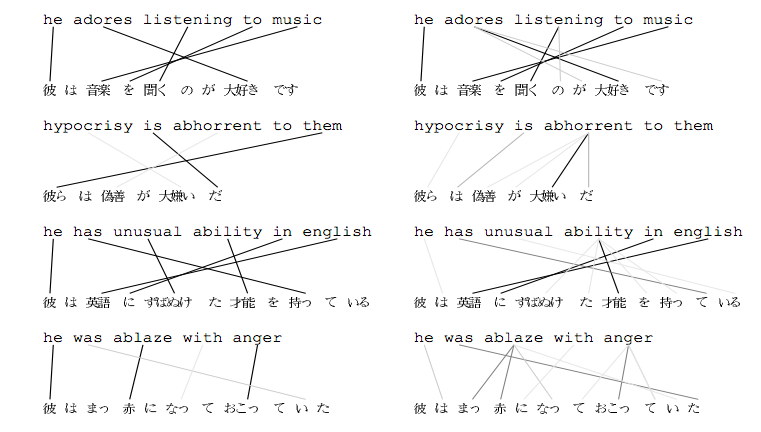
\includegraphics[width=\textwidth,,height=250pt]{figures/syntax1.png}
\caption{: Viterbi Alignments: Yamata et al's model (left) and IBM Model 5 (right). Darker lines are judged more
correct by humans.} \label{fig1}
\end{figure}

\begin{center}
\begin{tabular}{ |c|c|c| } 
 \hline & Alignment ave. score & Perfect sents \\ 
 \hline Yamata et al Model & 0.582 & 10 \\ 
 \hline IBM Model 5 & 0.431 & 0 \\ 
 \hline
\end{tabular}
\end{center}

\subsection{Moses and Factored Translation Model}
Moses is an open-source implementation of the statistical machine translation developed by Koehn et al (2007). The statistical machine translate systems are trained on huge quantities of parallel bilingual data and larger quantities of monolingual data. The parallel data is collection of sentences in two different languages which is sentence aligned, that is the sentence in one language is matched with sentence in corresponding language. In Moses, the system takes parallel data for the training process and uses the co-occurrences of phrases to infer translation correspondences between two languages of interest. In phrase-based machine translation, these correspondences are essentially between ceaseless arrangements of words, whereas in hierarchical phrase-based machine translation or syntax-based translation, more structure is added to the correspondences. Apart from being an open-source toolkit for SMT, Moses extended the phrase-based translation with factors and confusion network decoding. The phrase-based model in statistical machine translation was limited to the mapping of small text chunks with no express utilization of etymological data, be it morphological, syntactic, 
or on the other hand semantic. Previous researches showed that these additional sources of information are valuable when integrated into pre-processing or post-processing steps. Moses also integrated confusion network decoding, a mechanism which allowed translation of ambiguous input and enabled tighter integration of speech recognition and machine translation. The machine translation system examines a network of different word choices instead of passing along the one-best output of the recognizer. 
\subsubsection{Factored Translation Model}
The non-factored SMT such as phrase-based SMT typically dealt only with surface form of words and had one phrase table as shown in Figure 1. 
\begin{figure}
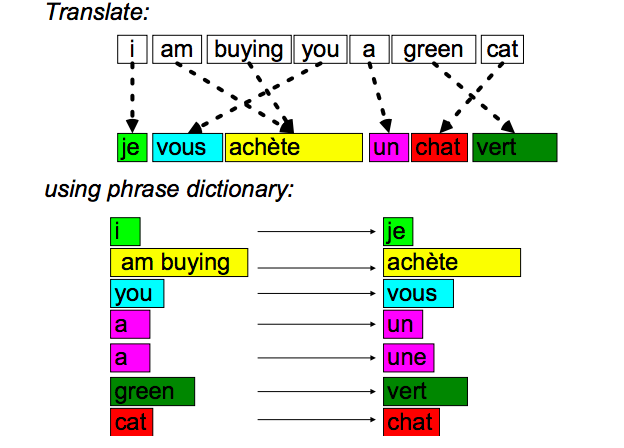
\includegraphics[width=\textwidth,,height=250pt]{figures/moses1.png}
\caption{Non-factored Translation} \label{fig1}
\end{figure}

In factored translation model, the surface forms may be augmented with different factors, such as POS tags or lemma. This creates a factored representation of each word, Figure 2 [Refer].
\begin{figure}
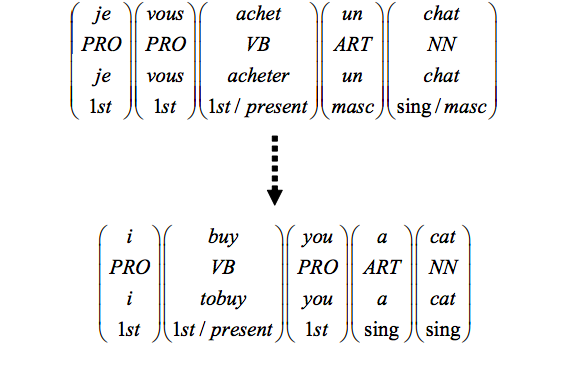
\includegraphics[width=\textwidth,height=250pt]{figures/moses2.png}
\caption{Factored Translation} \label{fig1}
\end{figure}

The authors suggested that mapping of source phrases to target phrases might be decomposed into a few stages. Decomposition of the decoding process into different steps implied that diverse components can be modelled independently. Modelling factors in isolation takes into consideration adaptability in their application. It can likewise increment accuracy and decrease sparsity by limiting the number conditions for each step. For example, a surface form can be decomposed to surface forms and lemma, as shown in figure3.
\begin{figure}
\begin{center}
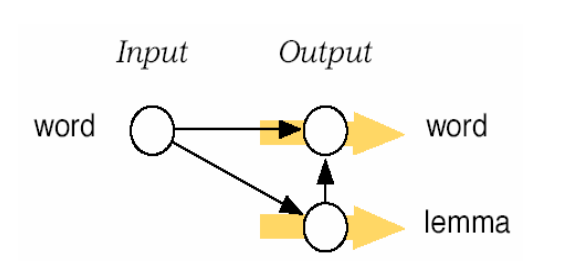
\includegraphics[width=300pt]{figures/moses3.png}
\caption{Example of graph of decoding systems} \label{fig1}
\end{center}
\end{figure}

The graph was allowed to be user definable, thus it provided a scope for experimentation with different configurations to find the optimum configuration for the given language pair and data. The authors considered the factors on the source sentence to be fixed, therefore they did not implement any decoding step to create source factors from other source factors. They designed Moses such as every factor on the target language could have its own language model.  Many factors such as lemmas and POS tags are sparser than surface forms so it was possible to create a higher order language models for these factors.

\subsubsection{Confusion Network Decoding}
The authors wanted to meet the increasing demands of integrating machine translation technology into bigger information processing systems with upstream NLP/speech processing tools such as named entity recognizers, speech recognizers, morphological analyzers, etc. The authors experimented with confusion networks by focusing on the speech translation case, where initially the input is generated by a speech recognition system. Their immediate goal was to improve the language translation by combining the speech recognition and machine translation models. The biggest problem in translation of spoken language was, its proneness to speech recognition errors which used to corrupt the input syntax and its meaning. Previous researches also showed that better translations can be obtained from the transcriptions of the speech recognizer.  The authors found that significant improvements could have been achieved by applying machine translation techniques on larger sets of transcription texts generated by the speech recognizers and combining the scores of acoustic models, language models, and translation models. 

In Moses, they implemented the confusing network decoding as discussed in (Bertoldi and Federico 2005), and they developed a simpler translation model and a more efficient implementation of the search algorithm.

\subsection{Challenges in SMT}

Statistical Machine Translation generated translation using statistical models whose parameters are derived from the analysis of bilingual text corpora. 

There were several challenges faced in statistical machine translation, which are as follows:

\begin{itemize}
    \item \textbf{Lack of Large Parallel Corpora}   Statistical Machine Translation systems need large sets of parallel data for the translation task. But the unavailability of large corpora in low resource language posed a challenge to the SMT and it affected the efficiency of translation models in several low resource languages.
    \item\textbf{Sentence Alignment }   In parallel corpora, a single sentence in one language when translated into other language may be more than one sentence, thus aligning such sentences in parallel becomes a challenge. Further, algorithms such as Gale-Church alignment algorithm needed to be used for sentence alignment.
     \item\textbf{Word Alignment }      Most of the popular parallel corpora is sentence aligned or sentence alignment can be done using the previously mentioned Gale-Church Algorithm. The real challenge lies for word alignment, to know which word in source language aligns with which word in the target language, though IBM models (Reference) and HMM-approach (Reference) provides a better solution to this problem.
     \item\textbf{Statistical anomalies }  Sometimes the real-world training sets tends to overwrite the translations of proper nouns. An abundance of particular noun in the training set may tend overwrite a less frequent noun in translated sentence. An example would be like,"\textit{Thóg mé an traein go Gaillimh} " in Irish should ideally translate to "\textit{I took the train to Galway}" in English, but gets to "\textit{I took the train to Cork"} due to abundance of "\textit{train to Cork}" in the training data.
     \item\textbf{Idioms }Depending upon the corpora utilized for the translation task, idioms may not translate "idiomatically". For instance, utilizing Canadian Hansard [Reference] as the bilingual corpus, "hear" may constantly be meant "Bravo!" since in Parliament "Hear, Hear!" moves toward becoming "Bravo!". 
     \item\textbf{Different Word Orders}    Different languages follow different word orders. In some languages, classification can be done by naming the typical order of subject (S), verb (V) and Object (O) in a sentence and in some languages, it can be represented as SVO or VSO. An example, the English sentence \textit{“Tom is eating vegetables”} is having the SVO word order, where as its translation in Hindi can be either \textit{“Tom vegetables kha raha hai”} which is SOV or \textit{“Vegetables kha raha hai Tom”} which is of the OVS order. 
     \item\textbf{Out of vocabulary (OOV) words}    The SMT systems typically store the different word forms as separate symbols which are unrelated to each other and words forms or phrases that were not in the training data which could not be translated. This is generally due to the lack of training data, changes in the human domain or some morphological differences. 
     \item\textbf{Mobile devices}   The rapid increase in the processing power of tablets and cell phones, combined with the wide accessibility of machine translation systems. However, combining other Speech recognition systems with SMT on mobile devices raises problems of sentence segmentation, de-normalization and punctuation prediction which is a basic necessity for quality translations.
\end{itemize}
\section{Neural Machine Translation Systems}
\subsection{Introduction}
\subsection{Google's Neural Machine Translation}
They proposed a model (see Figure \ref{gnmt1}) which follows the common sequence-to-sequence learning framework [41] with attention [2]. The model has three components: an encoder network, a decoder network and an attention network. The encoder network converts a source sentence into a list of vectors, one vector per input symbol. When this list of vectors is passed to decoder network it produces one symbol at a time until it encounters the special end-of-sentence symbol (EOS). The encoder and decoder are connected through an attention module which allows the decoder to focus on different regions of the source sentence during the course of decoding. 
\begin{figure}[h]
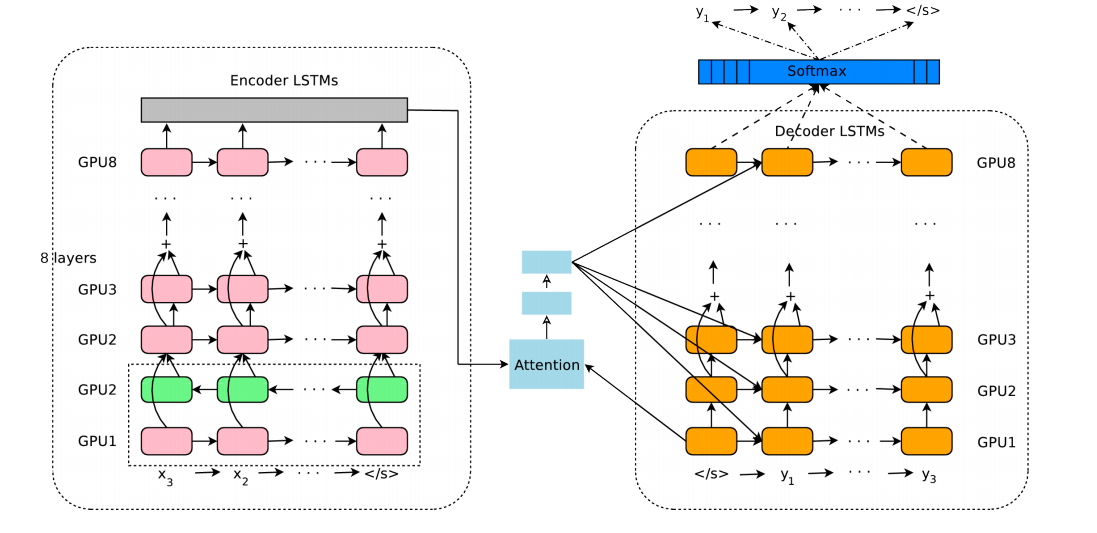
\includegraphics[width=\textwidth]{figures/gnmt1.png}
\caption{ The model architecture of GNMT, Google’s Neural Machine Translation system. } \label{gnmt1}
\end{figure}

On the left
is the encoder network, on the right is the decoder network, in the middle is the attention module. The
bottom encoder layer is bi-directional: the pink nodes gather information from left to right while the green
nodes gather information from right to left. The other layers of the encoder are uni-directional. Residual
connections start from the layer third from the bottom in the encoder and decoder. The model is partitioned
into multiple GPUs to speed up training. In our setup, we have 8 encoder LSTM layers (1 bi-directional layer
and 7 uni-directional layers), and 8 decoder layers. With this setting, one model replica is partitioned 8-ways
and is placed on 8 different GPUs typically belonging to one host machine. During training, the bottom
bi-directional encoder layers compute in parallel first. Once both finish, the uni-directional encoder layers
can start computing, each on a separate GPU. To retain as much parallelism as possible during running
the decoder layers, we use the bottom decoder layer output only for obtaining recurrent attention context,
which is sent directly to all the remaining decoder layers. The softmax layer is also partitioned and placed on
multiple GPUs. Depending on the output vocabulary size we either have them run on the same GPUs as the
encoder and decoder networks, or have them run on a separate set of dedicated GPUs.

For Notation, they used bold lower case to denote the vectors, bold upper case to denote the matrices, cursive upper case to denote the sets, capital letters to denote the sequences and lower case to denote the individual symbols in a sequence. 

They assumed (X,Y) as a source and target sentence pair , and $X$ = $x_1,x_2,x_3,..,x_M$ as the sequence of M symbols in the source text and $Y$= $y_1,y_2,y_3,.., y_N$ as the sequence of $N$ symbols in target text. The encoder is a simple function of the following form:
$$x_1,x_2,..,x_M = EncoderRNN(x_1,x_2,..,x_M)$$

Their decoder network is implemented as an amalgamation of an RNN network and a softmax Layer. The decoder RNN network creates a hidden state $Y_i$ for the next symbol to be predicted, which then goes through the softmax layer to generate a probability distribution over candidate output symbols. In their experiments the authors found out that Neural Machine Translation systems must have deep RNNs for encoder and decoder networks to achieve good accuracy, they need to capture the minute irregularities in the source and target languages. 

The Attention Model they implemented in their research is similar to [2]. More precisely, they assumed $y_{i-1}$ to be the decoder RNN from the previous decoding step which is the bottom decoder layer. Attention context $a_i$ , for the current time step is computed according to the following formulas:

\begin{align*}
    s_t &= AttentionFunction(y_{i-1},x_t)\;\forall t \;1\leq t\leq M\\
    p_t &= \frac{exp(s_t)}{\sum_{t=1}^M exp(s_t)}\;\forall t \;1\leq M\\
    a_i &= \sum_{t=1}^M exp(s_t) p_t.x_t
\end{align*}


Where \textit{AttentionFunction} in their implementation is a feed forward network with one hidden layer.

The authors acknowledged the fact that simply tacking up more Layers of LSTM makes the network slower and difficult to train, likely due to exploding and vanishing gradient problems [33,22]. The simple stacked LSTM layers work well up to 4 to 6 layers but performed very poorly beyond 8 layers.

\begin{figure}
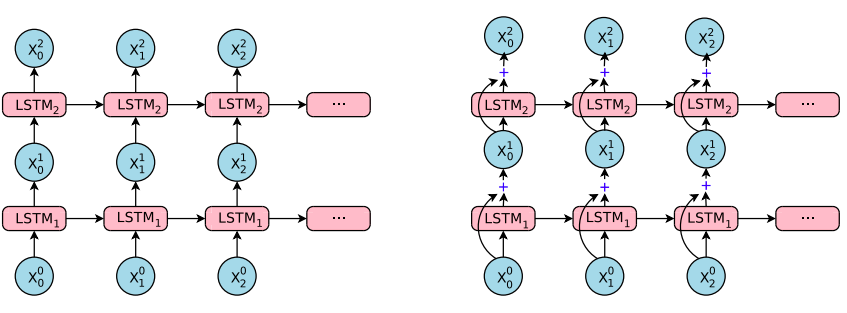
\includegraphics[width=\textwidth]{figures/gnmt2.png}
\caption{The difference between normal stacked LSTM and their stacked LSTM with residual connections.} \label{gnmt2}
\end{figure}

The authors were motivated by the idea of modelling differences between an intermediate layer’s output and the targets, which has shown to work well for many projects in the past [16,21,40], they introduced residual connections among the LSTM layers in a stack (See Figure \ref{gnmt2}). Residual Connection greatly improved the gradient flow in the backward pass, which allowed them to train their encoder and decoder networks with 8 LSTM layers. In translation systems, the information required to translate some words in the output language can appear anywhere in the source language. They decided to use a bi-directional RNN for the encoder to have the optimum scenario in the encoder network (See Figure \ref{gnmt3}). They used the bi-directional connections for the bottom encoder layer while keeping other layer uni-directional to allow maximum parallelization during computation. 

\begin{figure}
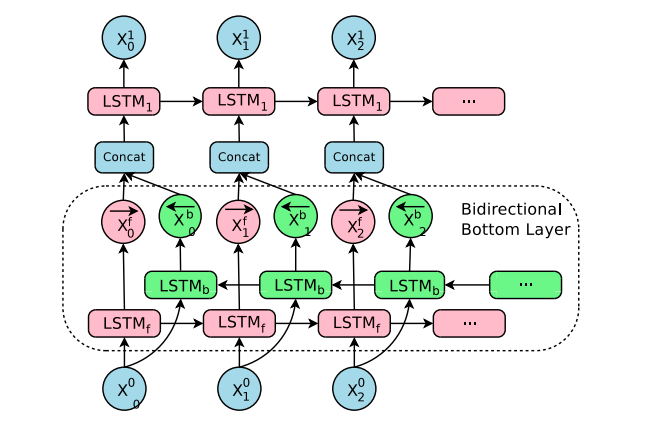
\includegraphics[width=\textwidth,height=250pt]{figures/gnmt3.png}
\caption{The structure of bi-directional connections in the first layer of the encoder. LSTM layer $LSTM_f$
processes information from left to right, while LSTM layer $LSTM_b$ processes information from right to left.
Output from $LSTM_f$ and $LSTM_b$ are first concatenated and then fed to the next LSTM layer $LSTM_1$.} \label
{gnmt3}\end{figure}

Due to the complexity of their model the authors implemented model parallelism and data parallelism to speed up the training. But Model Parallelism came up with certain constraints on their Model Architecture like they could not bi-directional LSTM layers for their all encoder layers.  The authors implemented the Wordpiece model which was initially developed by Google Speech Recognition System [35] for solving Japanese/ Korean segmentation problem to solve the out-of-vocabulary translation problems. 


\begin{figure}
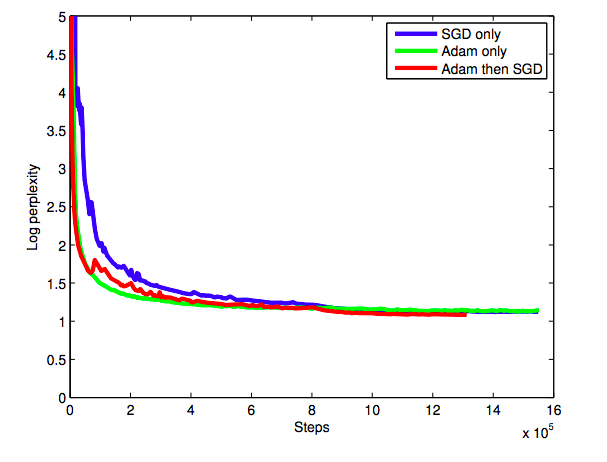
\includegraphics[width=\textwidth]{figures/gnmt5.png}
\caption{Log perplexity vs. steps for Adam, SGD and Adam-then-SGD on WMT En $\rightarrow$ Fr during maximum
likelihood training} \label{fig1}
\end{figure}

The authors used two publicly available corpora WMT’14 English-to-French (WMT En $\rightarrow$Fr) and English-to-German (WMT En $\rightarrow$De) as benchmarks for their Neural Machine Translation systems. In addition to these publicly available corpora they used Google’s translation production corpora which is much bigger than the WMT corpora for a given language pair. The WMT En-Fr contains 36M sentence pairs while the En-De contains 5M sentence pairs. They evaluated their models by carrying out side by side Human evaluations along with standard BLEU score metric. The side by side scores ranged from 0 to 6, with a score of 0 meaning “completely nonsense translation”, and a score of 6 meaning “perfect translation: the meaning of the translation is completely consistent with the source, and the grammar is correct”. They trained the models using the system they implemented in TensorFlow. For the initial stage of maximum likelihood training they used a combination of Adam [25] and SGD learning algorithms provided by TensorFlow. They ran Adam for the first 60K steps , after which they switched to simple SGD. They found that in the beginning Adam accelerates training but Adam alone converged to a worse point than a combination of Adam first, followed by SGD ( Figure 2.5). For the Adam part they used a learning rate of 0.0002 and for the SGD part they used a learning rate of 0.5. They used word-based, character-based, mixed-character-based and several wordpiece models with different vocabulary sizes for the experiments. Table summarizes the results they achieved on WMT En $\rightarrow$ Fr dataset. Their best model, WPM-32K achieved a BLEU score of 38.95. The WMT En $\rightarrow$ De was much more difficult than the En $\rightarrow$ Fr due to the less size of training data and German is a more morphologically rich language which needs vocabulary for word models. Their best model WPM-32K achieved a BLEU score of 24.61. 

\begin{table}[h!]
\centering
 \begin{tabular}{ |ccc| } 
  \hline Model & BLEU &  CPU decoding time
per sentence (s) \\ 
  \hline  Word &  37.90 & 0.2226\\
  Character (512 nodes)& 38.01 & 1.0530\\
  WPM-8K & 38.27 &  0.1919\\
  WPM-16K &  37.60 & 0.1874\\
  WPM-32K & 38.95 &  0.2118\\
  Mixed Word/Character & 38.39 &  0.2774\\
  \hline PBMT [15] & 37.0 &\\
  LSTM (6 layers) [31]  &  31.5 & \\
  LSTM (6 layers + PosUnk) [31] &33.1&\\
  Deep-Att [45] &  37.7&\\
  Deep-Att + PosUnk [45] &39.2\\
  \hline
 \end{tabular}
\caption{Results of the Single model on WMT En$\rightarrow$ Fr (newstest2014)}
\end{table}

\begin{table}[h!]
\centering
 \begin{tabular}{ |ccc| } 
  \hline Model & BLEU &  CPU decoding time
per sentence (s) \\ 
  \hline  Word &  23.12 & 0.2972\\
  Character (512 nodes)& 22.62 & 0.8011\\
  WPM-8K & 23.50 &  0.2079\\
  WPM-16K & 24.36 & 0.1931\\
  WPM-32K & 24.61 & 0.1882\\
  Mixed Word/Character & 24.17 & 0.3268\\
  \hline PBMT [6] & 20.7 &\\
  RNNSearch [37]  &  16.5 & \\
  RNNSearch-LV [37] &16.9&\\
  Deep-Att [45] & 20.6&\\
  \hline
 \end{tabular}
\caption{Results of the Single model on WMT En$\rightarrow$ De (newstest2014)}
\end{table}


They further used RL training to fine-tune the sentence BLEU score after normal maximum-likelihood training. The results of the best models showed that the fine-tuning of the models with RL can improve the BLEU scores. 


\begin{table}[h!]
\centering
 \begin{tabular}{ |ccc| } 
  \hline Dataset & Trained with log-likelihood &  Refined with RL \\ 
  \hline  En$\rightarrow$Fr &   38.95 & 39.92\\
  En$\rightarrow$De &  24.67 &  24.60\\
  \hline
 \end{tabular}
\caption{Single model test BLEU scores after RL Refining}
\end{table}

They ensembled 8 RL-refined models and obtained a state-of-the-art result of 41.6 BLEU points on the WMT En$\rightarrow$Fr dataset. They obtained a state-of-the-art result of 26.30 BLEU points on the WMT En$\rightarrow$De dataset. The results are showed in Table 3.4.For the side-by-side comparison, humans were asked to rate four translations for the given source sentence. The four translations were: 1) the best phrase-based translation downloaded from statmt website, 2) an ensemble of 8 ML-trained models, 3) an ensemble of 8 ML-trained and then RL-refined models, and 4) reference human translation directly obtained from test data. The results are showed in Table x.The results clearly showed that though RL refinement can achieve better BLEU scores, but it barely improved the human impression of the translation quality. 

\begin{table}[h!]
\centering
 \begin{tabular}{ |ccc| } 
  \hline Language & Model &  BLEU \\ 
  \hline  En$\rightarrow$Fr &   WPM-32K (8 models) & 40.35\\
  &RL-refined WPM-32K (8 models)& 41.16\\
  \hline
  En$\rightarrow$De &  WPM-32K (8 models) &  26.20\\
  &RL-refined WPM-32K (8 models)&26.30\\
  \hline
 \end{tabular}
\caption{Model ensemble results}
\end{table}




\begin{table}[h!]
\centering
 \begin{tabular}{ |ccc| } 
  \hline Model &  BLEU & Side-by-side
averaged score \\ 
  \hline PBMT [15]  &   37.0 & 3.87\\
  NMT before RL& 40.35&4.46\\
  NMT after RL&41.16& 4.44\\
  \hline
  Human &   &  4.82\\
  \hline
 \end{tabular}
\caption{Human side-by-side evaluation results for En$\rightarrow$Fr model}
\end{table}
They further carried out extensive experiments on many Google’s internal production data sets. As the experiments mentioned earlier carried doubts whether RL improves the real translation quality or simply the BLEU metric, they did not use model refinement for these experiments. The results obtained by the experiment showed that their model reduced translations by more than 60\% compared to the PBMT model on the major pairs of languages.


\subsection{OpenNMT}
OpenNMT is an open source framework for Neural Machine Translation developed by Harvard University and SYSTRAN. They designed OpenNMT with three aims: a) prioritize first training and test efficiency b) maintain model modularity and readability, c) support significant research extensibility. [Main OpenNMT] . 

They designed and developed  OpenNMT at Harvard, as a successor to $seq2seq-atn$, it was completely rewritten for ease of efficiency ,readability and generalizability. The OpenNMT framework includes the Vanilla NMT Models as well as provides support for attention, gating, stacking, input feeding, regularization, beam search and other options needed for State-of-the-art performance. They implemented the main system in the Lua/Torch mathematical framework which can be easily extended using Torch's internal neural network components. 

The authors designed the OpenNMT to meet certain goals: System Efficiency, code modularity and model extensibility. 

\begin{figure}
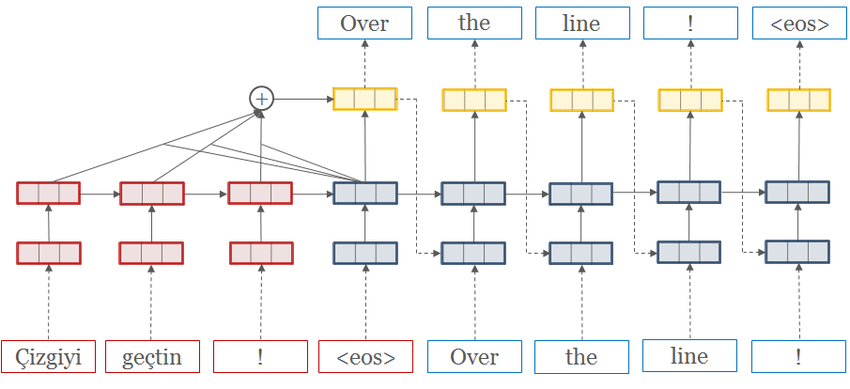
\includegraphics[width=\textwidth]{figures/openmt.png}
\caption{ Schematic view of neural machine translation. The red source words are first mapped to
word vectors and then fed into a recurrent neural network (RNN). Upon seeing the heosi symbol, the final
time step initializes a target blue RNN. At each target time step, attention is applied over the source RNN
and combined with the current hidden state to produce a prediction p(wt|w1:t−1, x) of the next word. This
prediction is then fed back into the target RNN} \label{fig1}
\end{figure}


\subsubsection{System Efficiency}

One of the biggest concerns about the Neural Machine Translation Systems is the training efficiency, the systems take huge time to train sometimes ranging from days to weeks. The authors tried to address the issue and tried to make the training slightly faster in OpenNMT. 

\textbf{Memory Sharing} The most common reason for high time consumption while training GPU-based NMT models is due to the memory size restrictions which limit the batch size. Though neural network toolkits like Torch has been designed to trade-off the surplus memory allocations for speed and declarative simplicity. For OpenNMT they implemented an external memory sharing system that utilizes the time-series control flow of NMT systems and vigorously shares the internal buffers between the clones. This implementation of vigorously memory reuse results in conservation of about 70\% of GPU memory with the default model size.

\textbf{Multi-GPU} The authors added support for multi-GPU training using data parallelism. Two modes were made available: synchronous and asynchronous training. In synchronous training, the batches run concurrently on parallel GPU and gradients aggregated to update master parameters before resynchronization on each GPU for the next batch. While in asynchronous training, the batches run independent on each GPU and independent gradients accumulated to the master copy of the parameters. Asynchronous SGD is known to provide faster convergence [Reference e (Dean et al., 2012). ] 

\textbf{C/Mobile/GPU Translation} The authors included several different translation models for different run-time environments in OpenNMT: a batched CPU/GPU implementation for quick translation of large set of sentences, a simple single-instance implementation for use on mobile devices and a specialized C implementation. 

\subsubsection{Modularity for Research}

The secondary goal for the authors were to make the code readable for non-experts and they targeted this goal by explicitly separating out optimizations from the core model and by including tutorial documentations within the code. 

Need to write here 

\textbf{Extensibility}

The field of Deep Learning is quickly evolving and technologies change very frequently. The authors went to perform different case studies to ensure that OpenNMT adhere to code extensibility and support the future variants.

Need to write a little more


\begin{table}[h!]
\caption{Performance Results for EN→DE on WMT15
tested on newstest2014. Both system 2x500 RNN, embedding
size 300, 13 epochs, batch size 64, beam size 5. We
compare on a 50k vocabulary and a 32k BPE setting. OpenNMT
showed improvements in speed and accuracy compared
to Nematus.\label{long}}
\centering
 \begin{tabular}{ |c|c|c|c|c| } 
 \hline Vocab & System & Speed Train & tok/sec Trans & BLEU \\ 
 \hline V=50K & Nematus & 3393 & 284 & 17.28 
 &&OpenNMT&4185&380&17.60\\ 
  \hline V=32K & Nematus & 3221 & 252 & 18.25 
 &&OpenNMT & 5254 & 457 & 19.34\\ 
 \hline
 \end{tabular}
\end{table}

\subsection{Nematus}

Nematus is an open source toolkit developed by Sennrich et al.(2017) from the Edinburgh NLP group, it is implemented in Python and based on the Theano framework (Theano Development Team, 2016) . They implemented an attentional encoder-decoder architecture which is similar to the one described by Bahadanau et al.(2015) , but there were several implementational differences.
\begin{itemize}
\item In the implementation of Nematus they initialized the decoder hidden state with the mean of the source annotation, rather than the annotation at the last position of the encoder backward RNN. 
\item They implemented a new conditional GRU with attention for Nematus.
\item In the decoder, they used a feedforward hidden layer with tanh non-linearity rather than a maxout before the softmax layer.
\item They didn’t implemented any additional biases for both encoder and decoder embedding layers.
\item The implementation of Bahadanau et al. (2015) used Look, Generate, Update decoder phases whereas in Nematus they implemented Look, Update, Generate which simplified decoder implementation significantly (See Table 1). 
\item They performed recurrent Bayesian dropout (Gal,,2015)
\item In Nematus they allowed multiple features (or “factors”) at each time step instead of a single word embedding at each source position, with the final embedding being the concatenation of the embeddings of each feature (Sennrich and Haddow, 2016).
\item They allowed tying of embedding matrices (Press and Wolf,2017;Inan et al.,2016).
\end{itemize}

\begin{table}[h!]
\centering
 \begin{tabular}{ |ll|ll|} 
 \hline
 \multicolumn{2}{|l|}{RNNSearch (Bahdanau et al., 2015)} & \multicolumn{2}{l|}{Nematus (DL4MT)}\\
  \hline  Phase & Output - Input & Phase & Output - Input \\
  \hline Look & $C_j$ $\leftarrow$ $S_{j-1}$ ,C & Look & $C_j$ $\leftarrow$ $S_{j-1}$, $Y_{j-1}$ ,C \\
  Generate & $Y_j$ $\leftarrow$ $S_{j-1}$, $Y_{j-1}$ ,$C_j$ & Update& $S_j$ $\leftarrow$ $S_{j-1}$, $Y_{j-1}$ ,$C_j$ \\
  Update & $S_j$ $\leftarrow$ $S_{j-1}$, $Y_{j}$ ,$C_j$ & Generate& $Y_j$ $\leftarrow$ $S_{j}$, $Y_{j-1}$ ,$C_j$ \\
  \hline
 \end{tabular}

\caption{Decoder phase differences between Nematus (DL4MT) and RNNSearch (Bahdanau et al., 2015)}
\end{table}

Given a source sequence ($x_1, . . . , x_T_x$ ) of length $T_x$ and a target sequence ($y_1, . . . , y_T_y$ ) of length $T_y$, let $h_i$ be the annotation of the source symbol at position $i$, obtained by concatenating the forward and backward encoder RNN hidden states, $h_i$ = [\overrightarrow{h_i} ; \overleftarrow{h_i} ], and $s_j$ be the decoder hidden state at position $j$.

\textbf{Decoder Initialization} Bahadanau et al. (2015) initialized the decoder hidden state $s$ with the last backward encoder state.
\begin{equation}
S_0 = tanh (W_{init}\overleftarrow{h_i})
\end{equation}

With $W_{init}$ as trained parameters. But in the Nematus implementation they used the average annotation instead:

\begin{equation}
S_0 = tanh (W_{init} \frac{\sum_{i=1}^{T_x}h_i}{T_x})
\end{equation}

\textbf{Conditional GRU with attention} Nematus implemented a novel conditional GRU with attention, $cGRU_{att}$. A $cGRU_{att}$ uses its previous hidden state $s_{j-1}$, the whole set of source annotations $C = {h_1, . . . , h_{T_x}}$ and the previously decoded symbol $y_{j-1}$ in order to update its hidden state $s_j$ , which is further used to decode symbol $y_j$ at position $j$.

\begin{equation}
s_j= cGRU_{att}(s_{j-1},y_{j-1},C)
\end{equation}


The conditional GRU layer with attention mechanism $cGRU_{att}$, consisted of three components : two GRU state transition blocks and an attention mechanism ATT in between. The first transition block, $GRU_1$, combines the previous decoded symbol  $y_{j-1}$ and previous hidden state $s_{j-1}$ in order to generate an intermediate representation $s_j^`$ with the following formulations:


\begin{align*}
s_j^` &= GRU_1(y_{j-1},s_{j-1})=(1-z_j^`)\bigodot \underline{s}_j^`+z_j^`\bigodot s_{j-1}^`,\\
\underline{s}_j^`&= tanh(W^`E[y_{j-1}]+r_j^`\bigodot(U^`s_{j-1})),\\
{r}_j^`&= \sigma (W_r^`E[y_{j-1}]+U_r^`s_{j-1}),\\
{z}_j^`&= \sigma (W_z^`E[y_{j-1}]+U_z^`s_{j-1}),
\end{align*}

, where $E$ is the target word embedding matrix, \underline{s}$_j^`$ is the proposal intermediate representation, $r_j^`$ and $z_j^`$ being the reset and update gate activation. In this formulation, $W^`$ , $U^`$ , $W_r^`$ , $U_r^`$ , $W_z^`$ , $U_z^`$ are trained model parameters; $\sigma$ is the logistic $sigmoid$ activation function.

In the Nematus implementation, the entire context set $C$ along with intermediate hidden state $s_j$ is taken as input in the attention mechanism ATT, in order to computer the context vector $c_j$ as follows:

\begin{align*}
c_j &= ATT(C,s_j^`)= \sum_{i}^{T_x}{a_{ij}}h_i\\
\alpha_{ij}&= \frac{exp(e_{ij})}{\sum_{k=1}^{T_x}exp(e_{kj})}\\
e_{ij} &= V_{\alpha}^T tanh(U_{\alpha}s_j^`+W__{\alpha}h_i)
\end{align*}
, where $\alpha_{ij}$ is the normalized alignment weight between source symbol at position $i$ and target symbol at position $j$ and $v_\alpha$, $U_\alpha$,$W_\alpha$ are the trained model parameters.

In the next step , $s_j$ is generated by the second transition block $GRU_2$ 

\begin{align*}
s_j^` = GRU_2(s_j^`,c_j)&=(1-z_j^`)\bigodot \underline{s}_j+z_j\bigodot s_{j}^`,\\
\underline{s}_j&= tanh(Wc_j+r_j\bigodot(Us_j^`)),\\
{r}_j&= \sigma (W_rc_j+U_rs_j^`),\\
{z}_j&= \sigma (W_zc_j+U_zs_j^`),
\end{align*}

, where \underline{s}$_j$ is the proposal hidden state, $r_j$ and $z_j$ being the reset and update gate activation. In this formulation, $W$ , $U$ , $W_r$ , $U_r$ , $W_z$ , $U_z$ are trained model parameters.

In Nematus, the two implemented GU blocks are not individually recurrent, they are only recurrent at the level of the whole cGRU layer. This way of combining RNN blocks is similar to what is referred in the literature as deep transition RNNs (Pascanu et al., 2014; Zilly et al., 2016) as opposed to the more common stacked RNNs (Schmidhuber, 1992; El Hihi and Bengio, 1995; Graves, 2013).

\textbf{deep output} Given $s_j , y_{j-1},$ and $c_j$ , the output probability $p(y_j|s_j , y_{j-1}, c_j )$ is computed by a softmax activation, using an intermediate representation $t_j$ . 

\begin{align*}
p(y_j|s_j , y_{j-1}, c_j ) = softmax (t_jW_o)\\
t_j=tanh (s_jW_{t1} + E[y_{j-1}]W_{t2} + c_jW_{t3}) \\
\end{align*}

,where $W_{t1},W_{t2},W_{t3},W_o$ are the trained model parameters.

They designed the Nematus to minimize the cross-entropy on parallel training corpus. For the training they used stochastic gradient descent, or one of its variants with adaptive learning rate (Adadelta (Zeiler, 2012), RmsProp (Tieleman and Hinton, 2012), Adam (Kingma and Ba, 2014)). Further, to optimize towards arbitrary, sentence level loss function they provided support for minimum risk training (MRT) (Shen et al., 2016). 

\begin{figure}
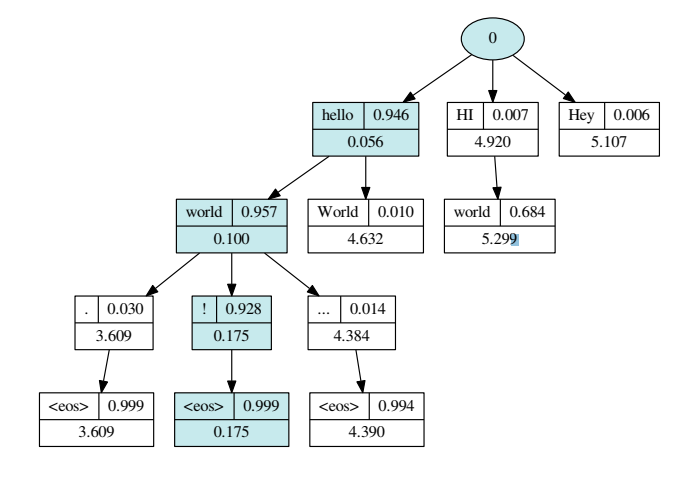
\includegraphics[width=\textwidth]{figures/nematus.png}
\caption{ Search graph visualisation for DE$\rightarrow$ EN
translation of "Hallo Welt!" with beam size 3 using Nematus} \label{fignm2}
\end{figure}

\subsection{Neural Monkey}
Neural Monkey is an open-source toolkit written using the TensorFlow machine learning library (Abadi et al., 2016). It provides a higher level API, such that it should be enough for the users to be familiar with the models on the equation level, without delving into implementation details. As compared to other open-source NMT toolkits, Neural Monkey provides a higher level of abstraction, along with a simple configuration mechanism that allows for fast prototyping and reusing trained models and experiment management.

The building blocks of Neural Monkey are not individual network layers like \textit{tfLearn} or \textit{Lasagne} , but they are more abstract objects like encoders and classifiers. These objects are parametrized so that their properties (e.g. number and sizes of hidden layers or dropout probability) can be set from a farther perspective. [Reference]. This design process allowed the authors to separate the configuration of the experiments from the actual code, which prevented the users from interleaving the configuration with other program logic. 

\begin{figure}
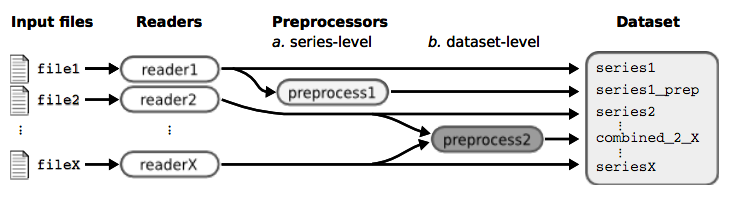
\includegraphics[width=\textwidth]{figures/nmonkey2.png}
\caption{ Creation of Dataset in Neural Monkey} \label{fignm2}
\end{figure}

In Neural Translation Systems, the loading and processing of datasets is one of the most important systems. The dataset in Neural Monkey is created in three step, first an input file is read using a Reader which load a file containing paths to JPEG images and load them as NumPy arrays, or read tokenized text as a list of lists of string tokens. The next phase is pre-processors, the series created by the readers is pre-processed by the system such as byte-pair encoding (Sennrich et al., 2016) which loads a list of merges and segments the text accordingly. Finally, the dataset-level pre-processors are applied of multiple series data to create the final dataset. 

\begin{figure}
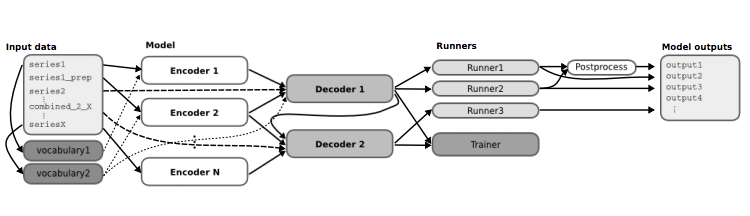
\includegraphics[width=\textwidth]{figures/nmonkey1.png}
\caption{ Model workflow in Neural Monkey} \label{fignm1}
\end{figure}


The model in Neural Monkey is defined by different model parts such as encoders and decoders. The authors defined the encoders and decoders in more general than the classical Sequence to Sequence Learning. They defined the Encoders as parts of the model which take the input and compute a representation of it. They used runners for the execution of the Decoders. They designed different runners to represent different ways of running the model. They implemented trainer which is a runner to modify the parameters of the model, to collect the objective functions and use them in a optimizer. They used an object called TensorFlow manager to manage all the TensorFlow sessions. 

In order to validate the Neural Monkey’s performance the authors did a sanity check evaluation on the architechture introduced by Bahadanau et al. (2014) which became the standard baseline model in NMT research. 








The used a bi-directional GRU network with 500 hidden units in each direction as the encoder and for decoder they used an RNN decoder with 1000 units in the hidden layer. They used a simple ‘tanh’ projection instead of max-out projection as used in the original model. The original paper used Adadelta (Zeiler, 2012) optimizer, whereas for this comparative study they used Adam (Kingma and Ba, 2014) . The comparison of the models is shown in Table. 

\begin{table}[h!]
\centering
 \begin{tabular}{ |c|c|c| } 
  \hline Model & BLEU & epoch \\ 
  \hline  Bahdanau et al.(2014) - neural & 26.75 & 2.2\\
  Bahdanau et al.(2014) - neural & 28.45 & 6.0\\
  SMT & 33.30 & -\\
  \hline Neural Monkey - greedy decoding & 25.08 & 1.2\\
  Neural Monkey + CGRU – greedy decoding  & 27.35 & 1.6\\
  \hline
 \end{tabular}
\caption{Results achieved by Neural Monkey on the WMT14 News Task French to English dataset with the number epochs}
\end{table}

\section{Related Work}
